% !TeX spellcheck = sk_SK-Slovak
\documentclass[slovak,10pt]{beamer}
% \documentclass[slovak, handout]{beamer}
\usepackage{newalg, wasysym, slashbox,lscape}
\usepackage{multirow}
\usepackage{multimedia}
\usepackage[normalem]{ulem}
%\usepackage{hyperref}
\usepackage{graphicx}
\usepackage{booktabs}
\usepackage{hhline}
\usepackage{xcolor}

\newcommand\coloreditem[1]{\item[\textcolor{#1}{\usebeamertemplate{itemize \beameritemnestingprefix item}}]}

\mode<presentation>
{
  \usetheme{Goettingen}
}

\usepackage{babel}
\usepackage[utf8]{inputenc}
%\usepackage[english]{babel}
% or whatever

%\usepackage[latin1]{inputenc}
% or whatever

\usepackage{times}
\usepackage[T1]{fontenc}
% Or whatever. Note that the encoding and the font should match. If T1
% does not look nice, try deleting the line with the fontenc.

\setbeamertemplate{headline}{\vskip10pt}
\setbeamertemplate{frametitle}{\insertframetitle\par\vskip-10pt}

%\usepackage{epsfig}
%\usepackage{pgf,pgfarrows,pgfnodes,pgfautomata,pgfheaps}

\title[Predikcia zhoršenia zdravotného stavu]{Predikcia zhoršenia zdravotného stavu}


\author[]{Marián Kravec \\ školiteľ: MSc. František Dráček }

\date{}

%\institute[]{Katedra Aplikovanej Informatiky\\ Fakulta Matematiky, Fyziky a Informatiky \\Univerzita Komensk\'eho}



% If you have a file called "university-logo-filename.xxx", where xxx
% is a graphic format that can be processed by latex or pdflatex,
% resp., then you can add a logo as follows:

% \pgfdeclareimage[height=0.5cm]{university-logo}{university-logo-filename}
% \logo{\pgfuseimage{university-logo}}

% Delete this, if you do not want the table of contents to pop up at
% the beginning of each subsection:
\AtBeginSection[]
{
  \begin{frame}<beamer>
    \frametitle{Obsah}
    \fontsize{9pt}{9pt}\selectfont
    \tableofcontents[currentsection,currentsubsection]
  \end{frame}
}


% If you wish to uncover everything in a step-wise fashion, uncomment
% the following command:

%\beamerdefaultoverlayspecification{<+->}
\beamerdefaultoverlayspecification{<+->}

% \newtheorem{Vysl}[theorem]{V�sledok}
% \newtheorem{Idea}[theorem]{My�lienka}

\def\ang#1{}

\begin{document}

\begin{frame}
  \titlepage
\end{frame}


% Since this a solution template for a generic talk, very little can
% be said about how it should be structured. However, the talk length
% of between 15min and 45min and the theme suggest that you stick to
% the following rules:

% - Exactly two or three sections (other than the summary).
% - At *most* three subsections per section.
% - Talk about 30s to 2min per frame. So there should be between about
%   15 and 30 frames, all told.

\section{Motivácia a ciele práce}

\begin{frame}{Motivácia a ciele práce}
	\begin{itemize}
		\item<1> Slovenské zdravotníctvo má nízku mieru využitia dostupných dát.
		\item<1> Predikcia budúcich nákladov pacienta môže zlepšiť plánovanie a prerozdelenie zdrojov.
		\item<1> Ciele:
		\begin{itemize}
			\item<1> Navrhnúť a implementovať spôsob transformácie záznamov pacienta do číselných vektorov (embedding).
			\item<1> Navrhnúť a implementovať systém na predikciu budúcich nákladov pacienta na základe jeho historických záznamov.
		\end{itemize}
		\item<1> Výsledky práce:
		\begin{itemize}
			\item<1> Embedované atribúty spĺňali vlastnosť blízkosti podobných záznamov.
			\item<1> Systém na predikciu budúcej nákladovej skupiny pacienta mal presnosť 39.9\% (84.4\% v prípade povolenia chyby o jednu kategóriu).
		\end{itemize}
	\end{itemize}
\end{frame}


\section{Dáta}

\begin{frame}  
	\frametitle{Dáta}
	\begin{itemize}
		\item<1> Umelo generované dáta podľa štruktúry NCZI: 173 355 pacientov, 133 miliónov záznamov.
		\item<1> Typ dát: poistné dáta.
		\item<1> Dve skupiny záznamov (datasety):
		\begin{itemize}
			\item<1> Výkony ambulantnej zdravotnej starostlivosti
			\item<1> Predpísané lieky
		\end{itemize}
		\item<1> Jeden záznam: informácia o jednom výkone/lieku konkrétneho pacienta.
		\item<1> Použité atribúty:
		\begin{itemize}
			\item<1> Dátum záznamu
			\item<1> Vek pacienta
			\item<1> Medicínsky výkon
			\item<1> Liek 
			\item<1> Diagnóza
			\item<1> Cena výkonu/lieku
		\end{itemize}
	\end{itemize} 
\end{frame}

\section{Embedding záznamov}

\begin{frame}{Vytváranie embeddingov záznamov}
	\begin{itemize}
		\item<1> Každý záznam reprezentovaný vektorom (embedding) z 4 častí:
		\begin{itemize}
			\item<1> Časová pečiatka (vek pri udalosti)
			\item<1> Diagnóza (MKCH-10, hierarchické embeddingy)
			\item<1> Liek (ATC, hierarchické embeddingy)
			\item<1> Výkon (LaBSE embedding popisu + PCA)
		\end{itemize}
		\item<1> Cieľ: podobné záznamy majú podobné vektory (Euclidovská vzdialenosť).
		\item<1> Overenie: klastrovanie, výpočty podobností.
	\end{itemize}
	\begin{center}
		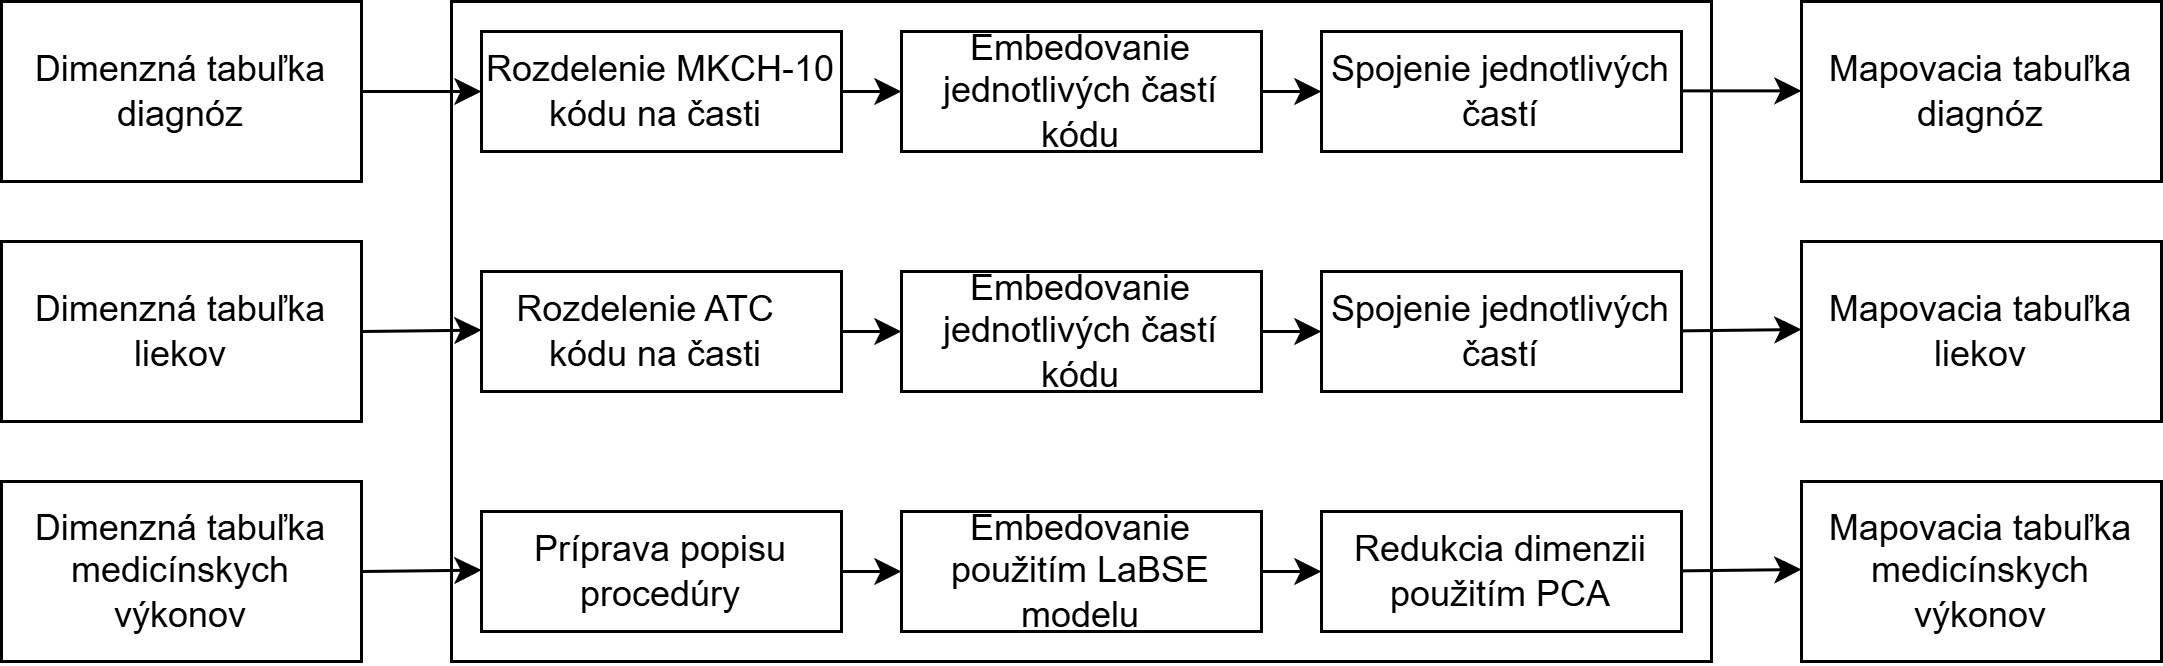
\includegraphics[height=3cm]{images/daig_emb_svk.png}
	\end{center}
\end{frame}

\begin{frame}
	\frametitle{Časová pečiatka}
	\begin{itemize}
		\item<1> Odhad veku pacienta v dňoch v čase záznamu.
		\item<1> Určená podľa veku pacienta v rokov v čase prvého záznamu a časovým rozdielom (v dňoch) medzi dátumami prvého a daného záznamu.
		\item<1> Chyba: v priemere štvrťrok, nanajvýš polrok.  
	\end{itemize}
\end{frame}

\begin{frame}
	\frametitle{Diagnózy}
	\begin{itemize}
		\item<1> Embedujeme MKCH-10 kódy.
	\end{itemize}

	\begin{center}
		
\includegraphics[height=0.6cm]{images/ICD_code.png}
	\end{center}
	\begin{itemize}
		\item<1> Hierarchický kód.
		\item<1> Každá časť kódovaná samostatne a následne spojené dohromady.
		\item<1> Príklad:
		\begin{itemize}
		\item<1> J - Choroby dýchacej sústavy
		\item<1> J3 - Iné choroby dýchacích ciest 
		\item<1> J38 - Choroba hlasiviek a hrtana
		\item<1> J38.0 - Obrna hlasiviek a hrtana
		\item<1> J38.01 - Jednostranná čiastočná obrna hlasiviek a hrtana
	\end{itemize}
	\end{itemize}

	\begin{center}
		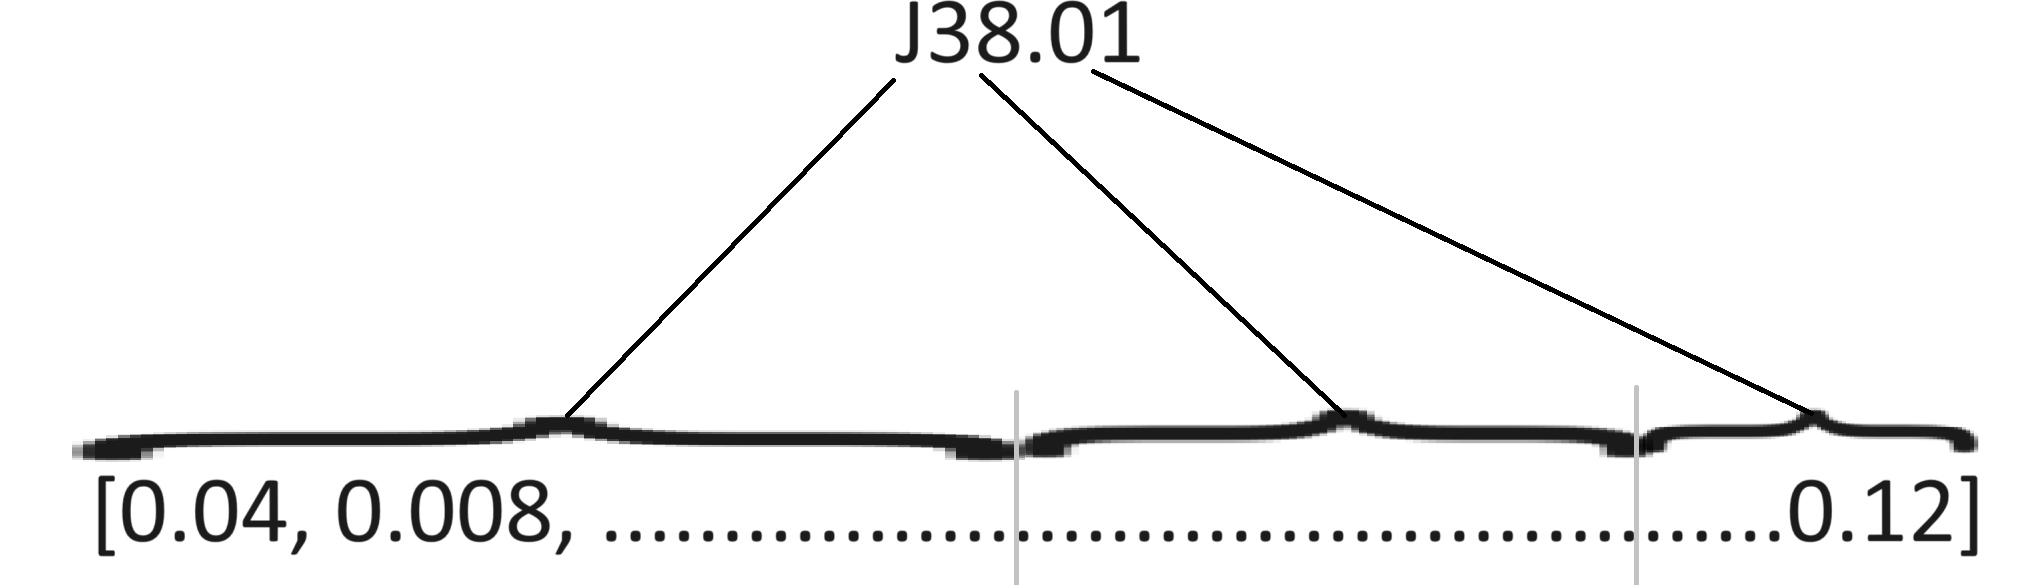
\includegraphics[height=1.6cm]{images/ICD_code_emb.png}
	\end{center}
\end{frame}

\begin{frame}
	\frametitle{Lieky}
	\begin{itemize}
		\item<1> Embedujeme ATC kód.
	\end{itemize}
	\begin{center}
		
\includegraphics[height=0.6cm]{images/ATC_code.png}
	\end{center}
	\begin{itemize}
		\item<1> Hierarchický kód.
		\item<1> Každá časť kódovaná samostatne a následne spojené dohromady.
		\item<1> Príklad:
		\begin{itemize}
			\item<1> N - Centrálna nervová sústava
			\item<1> N02 - Analgetiká
			\item<1> N02B - Iné analgetiká a antipyretiká
			\item<1> N02BA - Kyselina salicylová a deriváty
			\item<1> N02BA01 - Acylpyrín
		\end{itemize}
		
	\end{itemize}
	
\end{frame}

\begin{frame}
	\frametitle{Výkony}
	\begin{itemize}
		\item<1> Embedujeme textový popis výkonu.
		\item<1> Vyskúšané modely:
		\begin{itemize}
			\item<1> Language-agnostic BERT sentence embedding model (LaBSE)
			\item<1> Lemmatizer + Word2vec model
		\end{itemize}
		\item<1> Redukcia dimenzionality pomocou PCA, počet dimenzii vyberaný tak aby zachovávali 90\% variancie.
	\end{itemize}
	
\includegraphics[height=1.1cm]{images/vyk_flow.png}<1>
\end{frame}

% 7. Validácia embeddingov
\begin{frame}{Validácia embeddingov}
	\begin{itemize}
		\item<1> Diagnózy a lieky:
		\begin{itemize}
			\item<1> Porovnanie podobností (obrátená hodnota vzdialenosti) dvojíc niekoľkých náhodne vybraných prípadov.
			\item<1> Klastrovanie (K-means) a následné kontrola distribúcii hlavných kategórii prípadov v klastroch.
		\end{itemize}
		\item<1> Výkony: klastrovanie a následná vizuálna kontrola obsahu náhodne vybraných klastrov.
	\end{itemize}
\end{frame}

% 7. Validácia embeddingov
\begin{frame}{Validácia embeddingov}
	\begin{columns}[T]%{cl}  
		\begin{column}{.48\textwidth}<1->%{c}
			Diagnózy 
			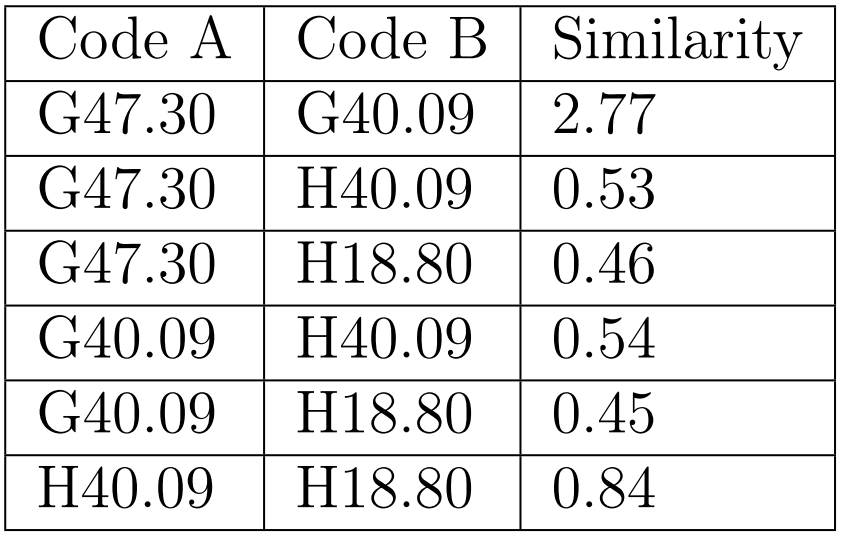
\includegraphics[height=2.8cm]{images/diag_sim.png}<1>
			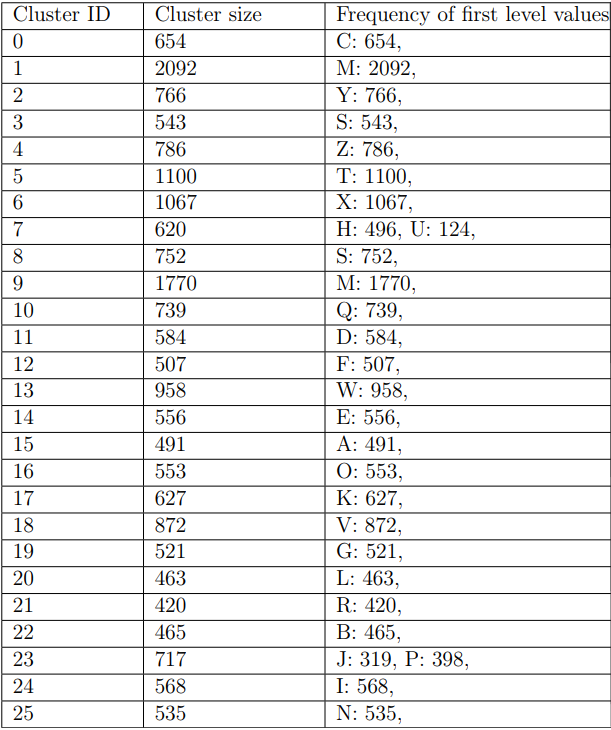
\includegraphics[height=6.2cm]{images/diag_clust.png}<2>
			
		\end{column}
		%&
		\hfill%
		\begin{column}{.48\textwidth}<1->%{l}
			Lieky 
			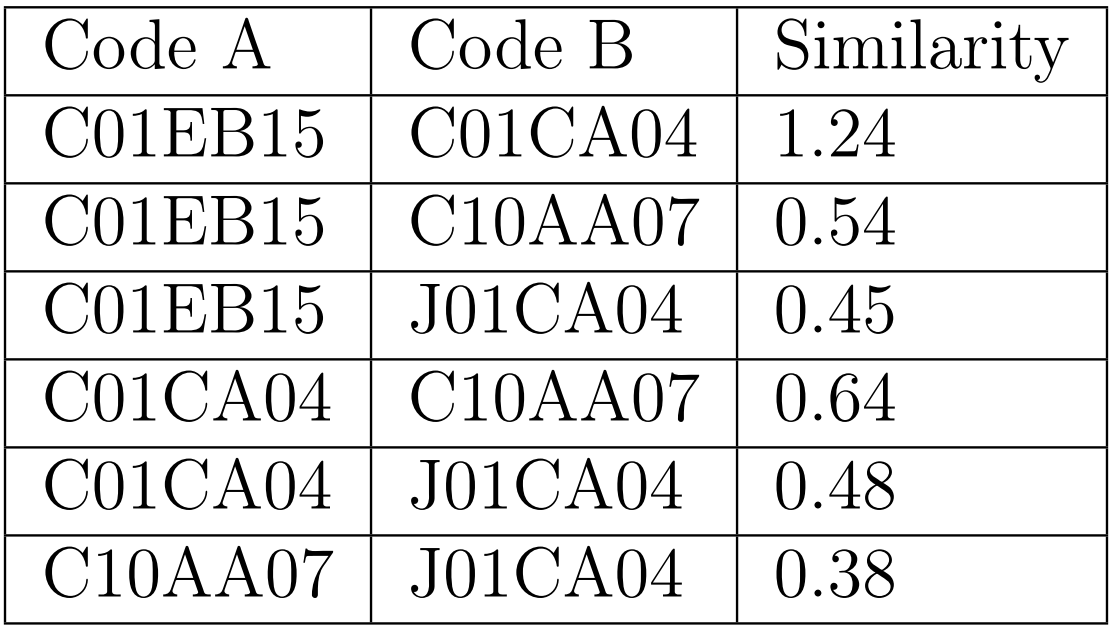
\includegraphics[height=2.8cm]{images/drug_sim.png}<1>
			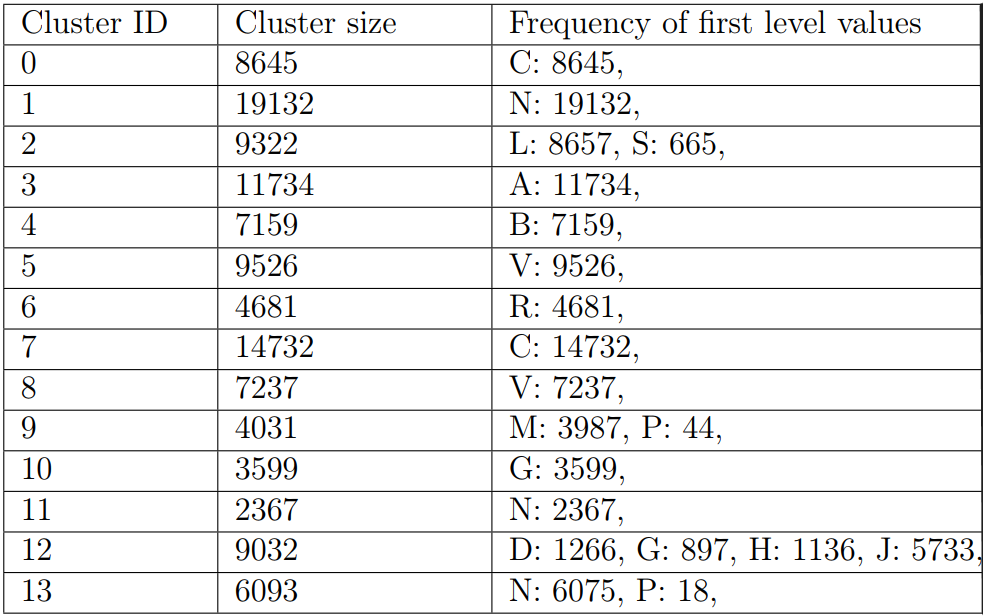
\includegraphics[height=3.1cm]{images/drug_clust.png}<2>
			
		\end{column}  
	\end{columns}
\end{frame}

\begin{frame}{Validácia embeddingov}
	Medicínske výkony
	\begin{itemize}
		\item<1> Kluster 215:
		\\
		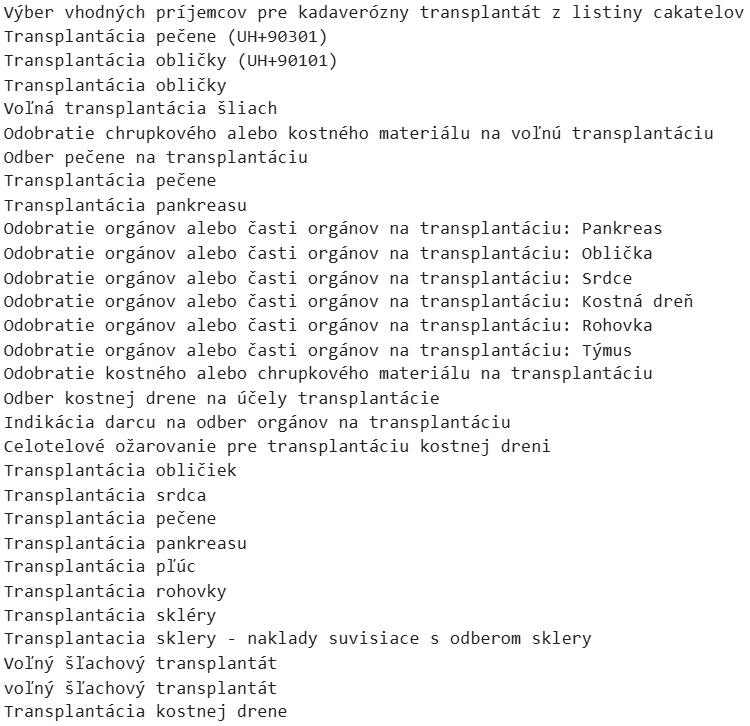
\includegraphics[height=6.5cm]{images/G215.png}<1>
		\item<2> Kluster 45:
		
\includegraphics[height=4.3cm]{images/G45.png}<2>
	\end{itemize}
	%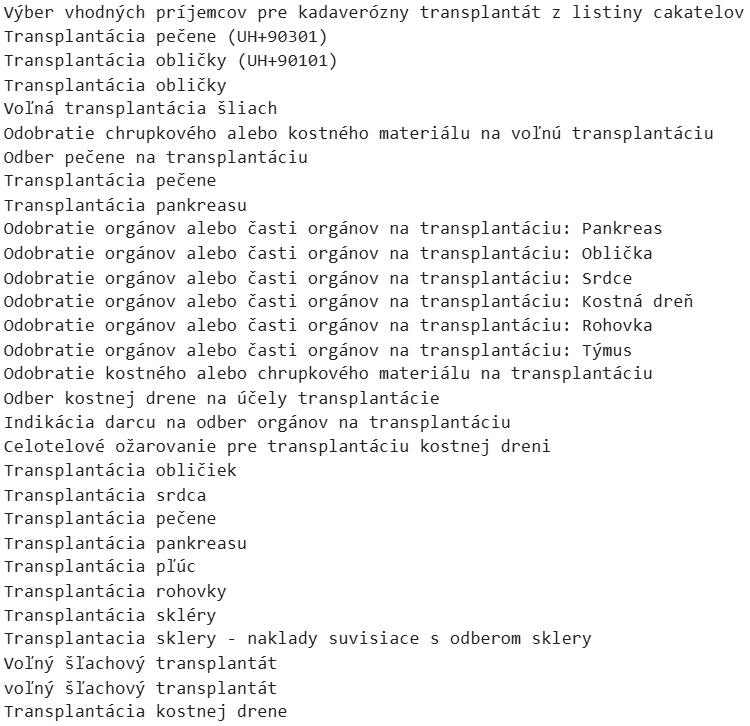
\includegraphics[height=4cm]{images/G215.png}<1>
	%
\includegraphics[height=2.6cm]{images/G45.png}<1>
	
\end{frame}


\section{Predikcia budúcich nákladov na pacienta}

\begin{frame}
	\frametitle{Proces predikcie}
	\begin{itemize}
		\item<1> Kroky pri predikovaní budúcej cenovej kategórie pacienta:
		\begin{enumerate}
			\item<1> Načítanie dát pacienta, embedding a normalizácia.
			\item<1> Výpočet počtu záznamov na budúci rok.
			\item<1> Predikcia budúcich záznamov.
			\item<1> Predikcia cenových kategórii budúcich záznamov.
			\item<1> Výpočet cenovej kategórie pacienta.
		\end{enumerate}
		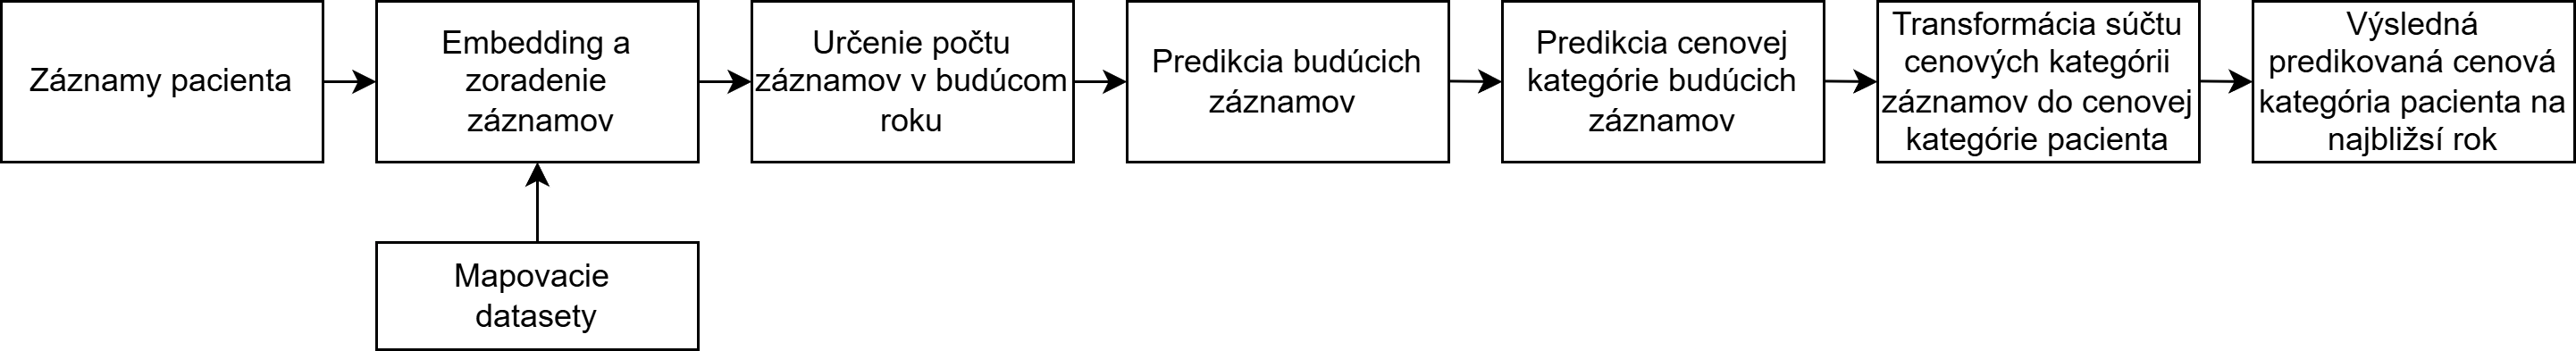
\includegraphics[height=1.25cm]{images/system_flow.png}
		\item<1> Hyperparametre modelov nastavované lokálne na podskupine pacientov.
		\item<1> Finálne modely trénované na serveri na plnohodnotnom datasete.
	\end{itemize}
\end{frame}

\begin{frame}
	\frametitle{Výpočet počtu budúcich záznamov}
	\begin{itemize}
		\item<1> Testované metódy:
		\begin{itemize}
			\item<1> Polynomialna regresia počtu záznamov z predchádzajúcich rokov.
			\item<1> Generovanie nových záznamov kým generovaná časová pečiatka nepresiahne rok od posledného skutočného záznamu.
		\end{itemize}
		\item<1> Najlepší výsledok: lineárna regresia.
	\end{itemize}
	\begin{center}
		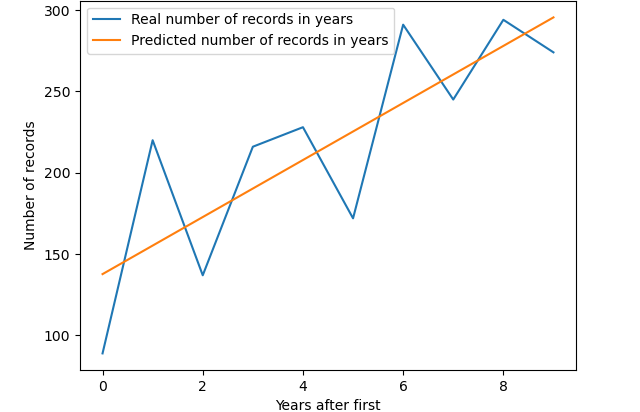
\includegraphics[height=4.5cm]{images/num_of_rec.png}
	\end{center}
\end{frame}

\begin{frame}
	\frametitle{Predikcia budúcich záznamov}
	
	\begin{columns}[T]%{cl}  
		\begin{column}{.56\textwidth}<1->%{c}
			\begin{itemize}
				\vspace{0.2cm}
				\item<1> Testované modely:
				\begin{itemize}
					\item<1> Long short-term memory.
					\item<1> Decoder-only transformer.
				\end{itemize}
				\item<1> Vstup: posledných $n$ (veľkosť okna/kontextu) záznamov pacienta.
				\item<1> Výstup: predikcia nasledujúceho záznamu.
				\item<1> Chybová funkcia: Subpart weighted MSE\\
				
\includegraphics[height=0.8cm]{images/swMSE.png}
				\item<1> Optimalizované hyperparametre: 
				\begin{itemize}
					\item<1> Hĺbka modelu (počet vrstiev).
					\item<1> Šírka modelu (LSTM).
					\item<1> Počet hláv (Transformer).
					\item<1> Dropout rate.
				\end{itemize}
			\end{itemize}
		\end{column}
		%&
		\hfill%
		\begin{column}{.42\textwidth}<1->%{l}
			\begin{center}
				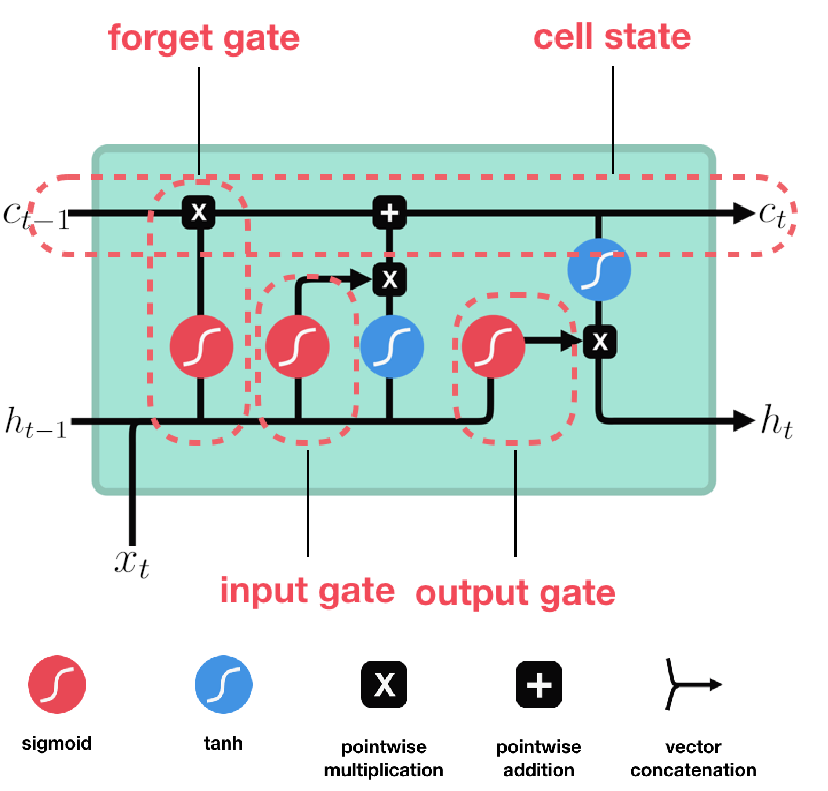
\includegraphics[height=3.2cm]{images/LSTM_arch.png}
			\end{center}
			\begin{center}
				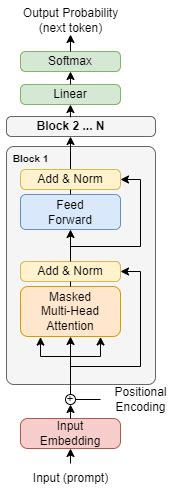
\includegraphics[height=4.3cm]{images/decod_only_trans_arch.png}
			\end{center}
		\end{column}  
	\end{columns}
\end{frame}

\begin{frame}
	\frametitle{Predikcia budúcich záznamov - trénovanie a validácia}
	
	\begin{columns}[T]%{cl}  
		\begin{column}{.42\textwidth}<1->%{c}
			LSTM
			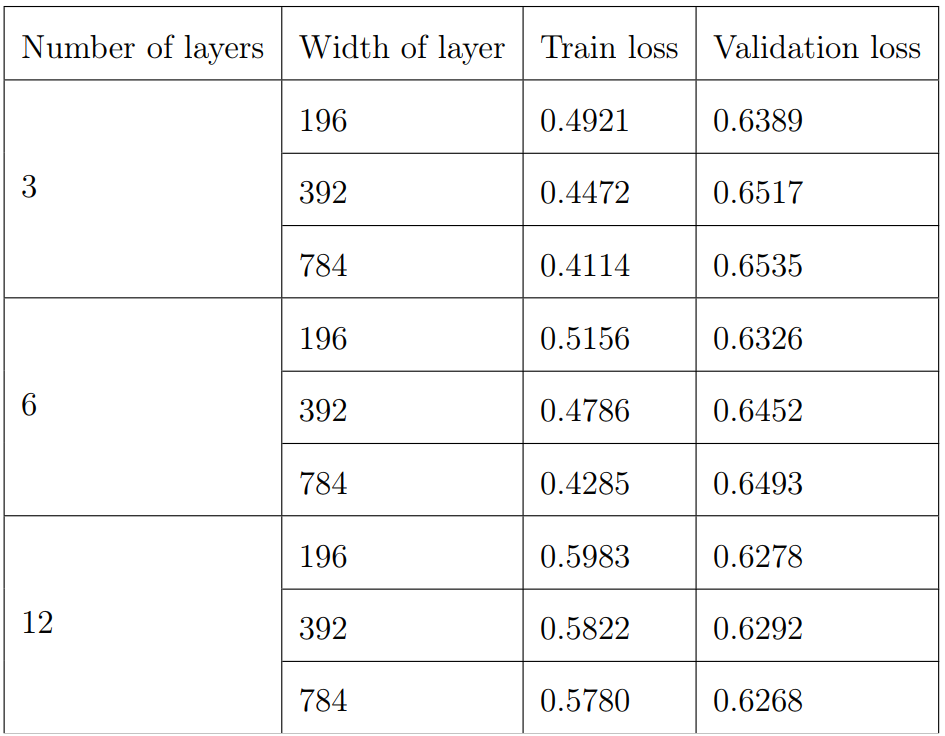
\includegraphics[height=3.85cm]{images/train_LSTM.png}
		\end{column}
		%&
		\hfill%
		\begin{column}{.49\textwidth}<1->%{l}
			Transformer
			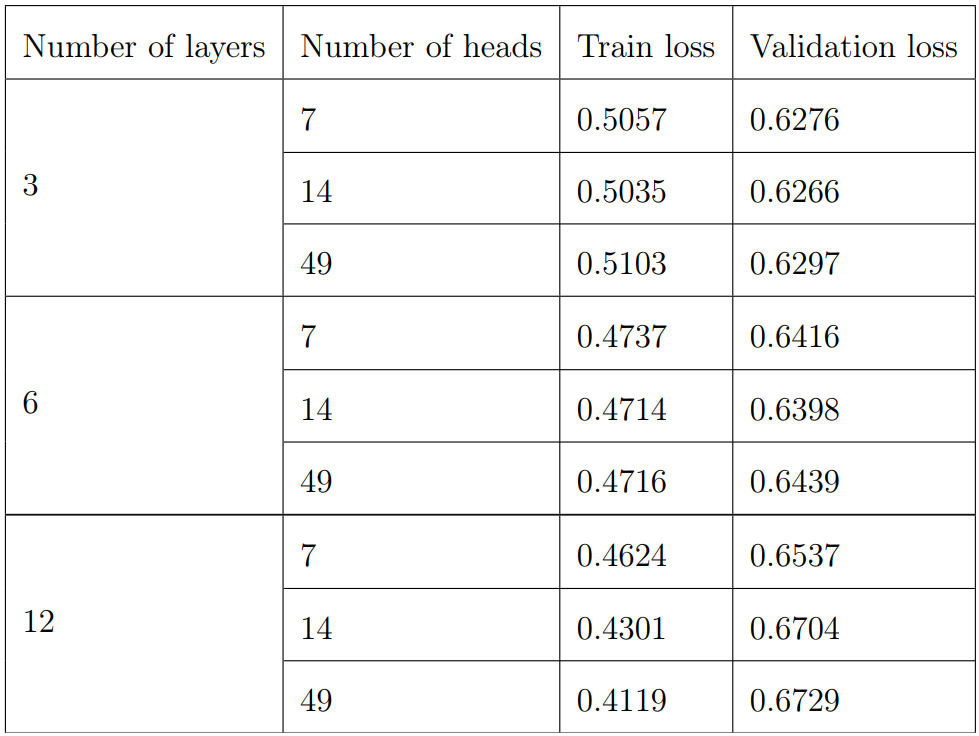
\includegraphics[height=3.85cm]{images/train_Trans.png}
		\end{column}  
	\end{columns}
	\begin{itemize}
		\item<1> Najlepší model pri lokálnom trénovaní: Decoder-only Transformer, 3 vrstvy, 14 hláv, 20\% dropout rate.
		\item<1> Chyba pri trénovaní na serveri: 
		\begin{itemize}
			\item<1> Trénovacia: 0.4005
			\item<1> Validačná: 0.5200
		\end{itemize}
	\end{itemize}
\end{frame}

\begin{frame}
	\frametitle{Predikcia cenovej kategórie záznamu}
	\begin{itemize}
		\item<1> Použitý model: Multilayer perceptron.
		\item<1> Vstup: jeden záznam pacienta.
		\item<1> Výstup: jedna z 9 cenových kategórii.
		\item<1> Vyskúšané jednoduchšie modely: Gradient boosting, Ridge regression
	\end{itemize}
	\begin{columns}[T]%{cl}  
		\begin{column}{.64\textwidth}<1->%{c}
			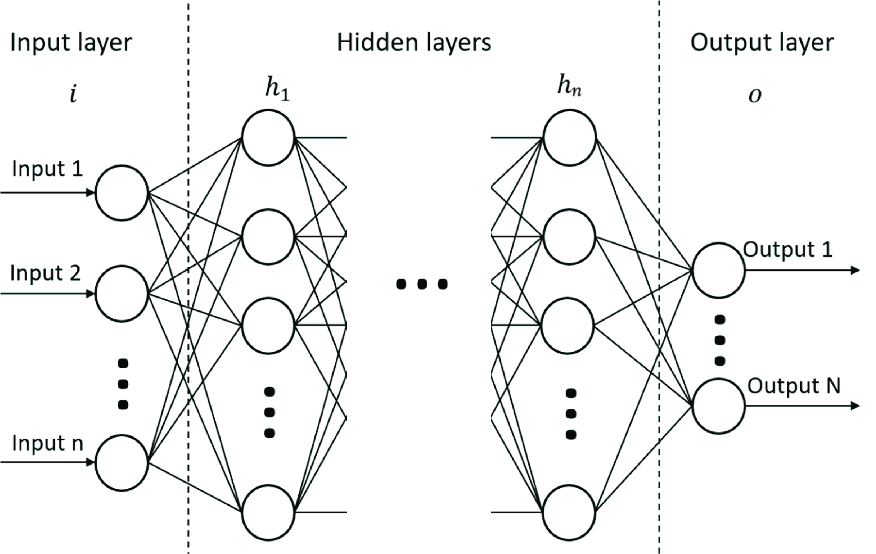
\includegraphics[height=4cm]{images/MLP_arch.png}
		\end{column}
		%&
		\hfill%
		\begin{column}{.32\textwidth}<1->%{l}
			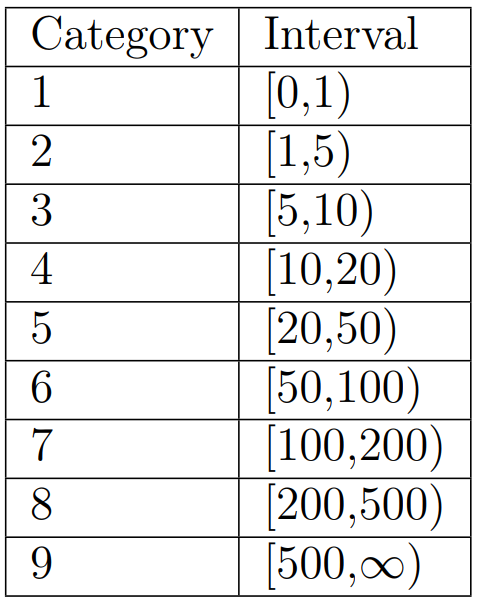
\includegraphics[height=4cm]{images/mlp_cat.png}
		\end{column}  
	\end{columns}
\end{frame}

\begin{frame}
	\frametitle{Predikcia cenovej kategórie záznamu - trénovanie a validácia}
	\begin{itemize}
		\item<1> Optimalizované hyperparametre:
		\begin{itemize}
			\item<1> Hĺbka modelu.
			\item<1> Veľkosti jednotlivých vrstiev.
			\item<1> Aktivačné funkcie medzi vrstvami.
			\item<1> Chybová funkcia (MSE, Cross Entropy, NLL).
		\end{itemize}
		\item<1> Miera kvality modelu: presnosť.
	\end{itemize}
	\begin{center}
		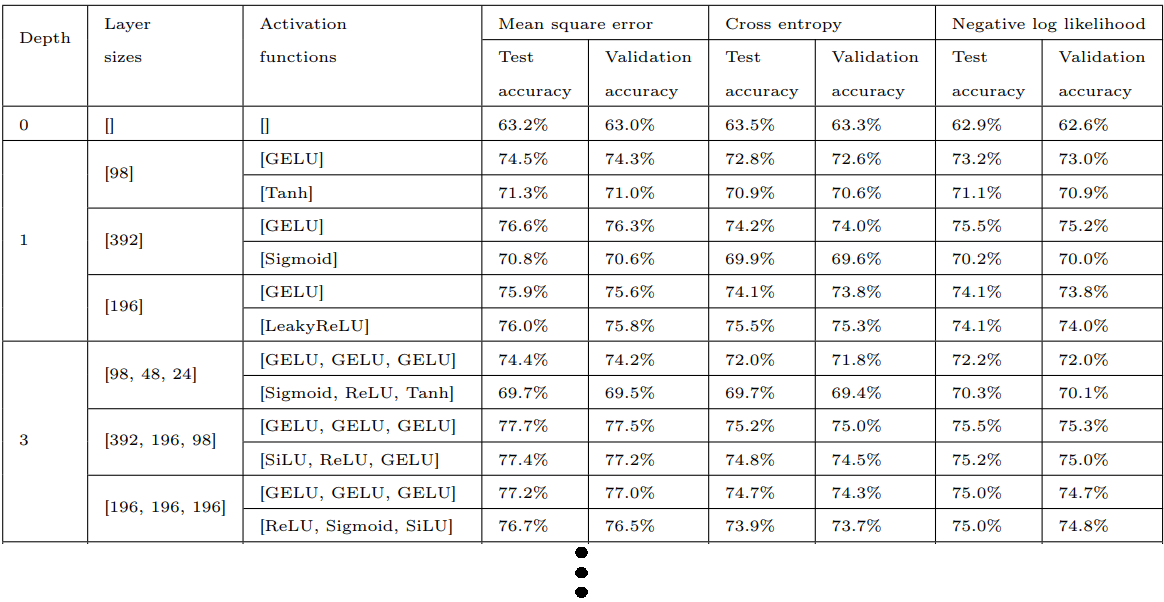
\includegraphics[height=4.5cm]{images/MLP_train.png}
	\end{center}
		
\end{frame}

\begin{frame}
	\frametitle{Predikcia cenovej kategórie záznamu - trénovanie a validácia}
	\begin{itemize}
		\item<1> Najlepší model pri lokálnom trénovaní:
		\begin{itemize}
			\item<1> 8 vrstiev.
			\item<1> Šírky vrstiev: [588, 294, 147, 49, 98, 36, 18, 9].
			\item<1> Aktivačné funkcie medzi vrstvami: [SiLU, GELU, Sigmoid, GELU, SiLU, GELU, LeakyReLU, Softmax].
			\item<1> Chybová funkcia: MSE.
		\end{itemize}
		
		\item<1> Presnosť pri lokálnom trénovaní: 
		\begin{itemize}
			\item<1> Trénovacia: 78.3\%
			\item<1> Validačná: 78.0\%
		\end{itemize}
		\item<1> Presnosť pri trénovaní na serveri: 
		\begin{itemize}
			\item<1> Trénovacia: 80.2\%
			\item<1> Validačná: 80.1\%
		\end{itemize}
		\item<1> Validačná presnosť najlepšieho Gradient boosting: 71.4\%
		\item<1> Validačná presnosť najlepšieho Ridge regression: 66.9\%
	\end{itemize}
	
\end{frame}

\begin{frame}
	\frametitle{Predikcia cenovej kategórie pacienta - validácia}
	\begin{columns}[T]%{cl}  
		\begin{column}{.44\textwidth}<1->%{c}
			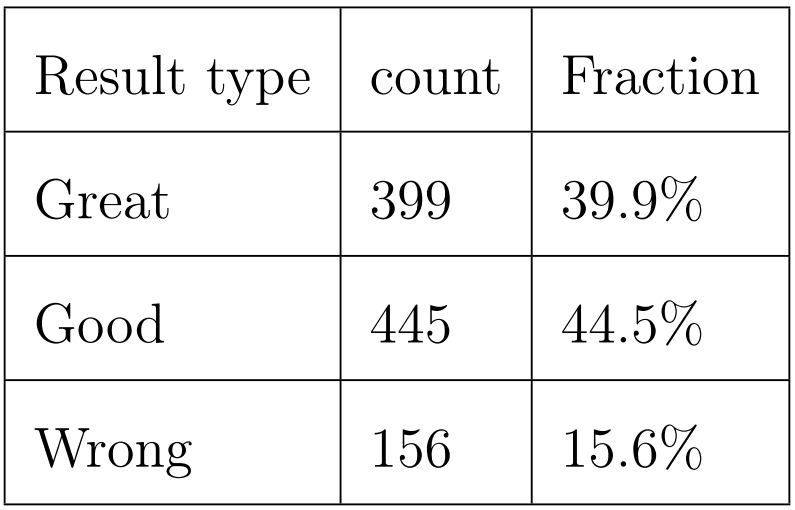
\includegraphics[height=3.46cm]{images/tot_res_1.png}
			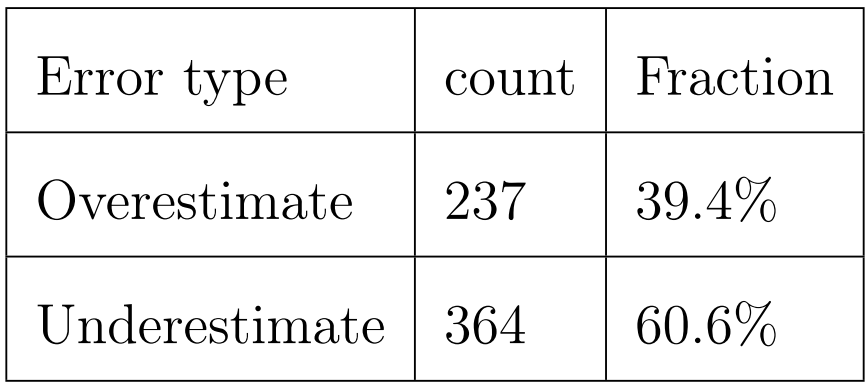
\includegraphics[height=2.4cm]{images/tot_res_2.png}
		\end{column}
		%&
		\hfill%
		\begin{column}{.32\textwidth}<1->%{l}
			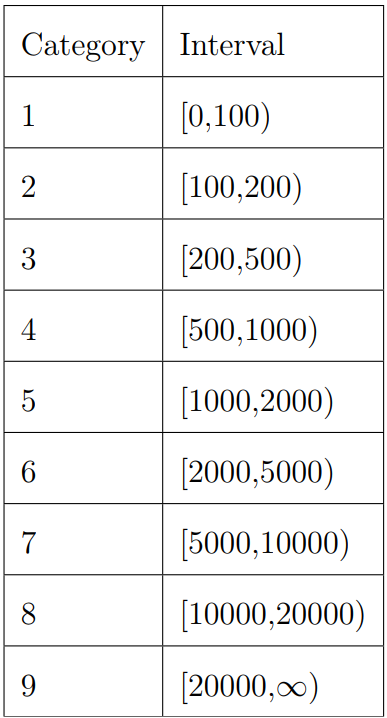
\includegraphics[height=6.4cm]{images/tot_cat.png}
		\end{column}  
	\end{columns}
\end{frame}


\begin{frame}
	\frametitle{}
	
	\large{Ďakujem za pozornosť}
\end{frame}

\section{Príprava na otázky s posudkov}

\begin{frame}
	\frametitle{}

	
\includegraphics[height=7cm]{images/thesis_defense_2x.png}<1>
	zdroj: XKCD (\url{https://xkcd.com/1403/})
\end{frame}

\end{document}
